A continuación se expondrá brevemente el uso de tecnologías así como la metodología
de trabajo que se ha seguido para la elaboración de la aplicación.

\section{Herramientas y tecnologías usadas}

\subsection{Django - Django Channels}

Las bases del proyecto se fundamentan en el uso de Django \cite{django} como tecnología de backend.

Además de conocer en profundidad cómo funcionan este framework y Python (que es el lenguaje con el que trabaja Django),
esta se trata de una herramienta que permite un desarrollo rápido y escalable.

Por otra parte se trabajará con Django Channels \cite{djangoChannels} para gestionar el uso de websockets. Django Channels
permite el uso de websockets y tecnologías análogas mediante varios paquetes que se integran dentro del framework de Django.
A través del uso de ``consumers'' o consumidores, abstracciones propias de Channels, 
se desarrollará la mayor parte de la lógica de la aplicación. 

Posteriormente se hará mención a Pytest \cite{pytest} a la hora de implementar el testing automático.

\subsection{Vue3}

Por otro lado, para el desarrollo frontend se propone el uso de Vue \cite{vue3} debido a su popularidad, versatilidad
y a su uso personal en otros proyectos. De esta forma se creará un frontend sencillo pero bastante personalizable.

Se hace referencia a Vue3 por ser la versión más moderna de Vue, la cual tiene cambios destacables en comparación
a Vue2 \cite{vue3vue2}. Todos los paquetes y librerías adicionales se incorporarán teniendo en cuenta que se está haciendo uso de
Vue3. En especial, se destaca la librería de componentes Vuetify \cite{vuetify}, la cual es un gran añadido a la hora de
ofrecer una gran diversidad de componentes para la construcción de una interfaz vistosa y dinámica.

\subsection{Herramientas de diseño}

Figma \cite{figma} es un editor de gráficos que se usa principalmente para generar prototipos. Se usará principalmente para
el diseño y experimentación inicial de la aplicación web. Además de Figma, se harán uso de otras herramientas
menores de diseño como draw.io \cite{draw.io} para la creación de diagramas, Pictogrammers \cite{pictogrammers} para hacer uso de
iconos de forma sencilla o Contrast Finder \cite{contrastFinder} para comparar contrastes de color.

\subsection{Docker}

Docker \cite{docker} es una herramienta de código abierto que facilita un despliegue sencillo y portable utilizando contenedores. 
Un contenedor es una unidad estándar de software que agrupa el código y todas sus dependencias para que la aplicación se ejecute de 
manera rápida y fiable en diferentes entornos de computación \cite{dockerContainer}. Con el uso de Docker, se preparará la aplicación 
en diferentes contenedores para su despliegue de forma sencilla.

\subsection{AWS}

Amazon Web Services (AWS)~\cite{aws} es una plataforma de servicios en la nube ofrecida por Amazon. Proporciona
una amplísima gama de servicios que incluyen computación, almacenamiento, bases de datos, etc. Estas soluciones permitirán
alojar la aplicación final de forma flexible.

Se detallará el uso tanto de Docker como de AWS en el proceso de preparación y despliegue de la aplicación.

\subsection{GitHub}

GitHub \cite{github} es una plataforma de desarrollo colaborativo basada en la web que utiliza Git, un sistema de control de versiones
distribuido. Permite a los desarrolladores alojar, gestionar y compartir proyectos de software, facilitando la accesibilidad
del código.

Todo el código del proyecto será accesible mediante un repositorio público en GitHub \cite{repositorio} .

\subsection{WSL}

Se destaca de forma adicional el uso del subsistema de Windows para Linux (WSL) \cite{wsl} para poder ejecutar de forma sencilla
todo el entorno de la aplicación así como para la realización de pruebas de despliegue sin dejar de hacer uso directo de Windows
como sistema operativo.

\subsection{Visual Code}

En último lugar se encuentra la herramienta más básica y a la vez más importante para
el proyecto, Visual Studio Code \cite{vscode}. Visual Studio Code, comúnmente conocido como Visual Code o VS Code,
es un editor de código fuente desarrollado por Microsoft.

Todo el código se ha tratado mediante Visual Code, desde la creación y edición del código hasta la ejecución de comandos
en la terminal del sistema.


\section{Metodología}

Este proyecto se ha guiado por el uso de una metodología de trabajo iterativa-incremental enfocada en la revisión de objetivos y
avances entre el tutor y el alumno. Durante cada encuentro, se han ido discutiendo propuestas de mejora que se han convertido en
objetivos para la siguiente evaluación. En primera instancia, después de 
plantear los objetivos principales del desarrollo y la motivación general
del proyecto, se han propuesto tres diferentes fases de progreso con fechas estimadas:

\begin{itemize}
	\item Fase 1: Septiembre 2023 - Diciembre 2023
	\item Fase 2: Enero 2024 - Febrero 2024
	\item Fase 3: Marzo 2024 - Mayo 2024
\end{itemize}

En la primera fase se destaca como objetivo principal crear una primera versión sencilla de la aplicación con 
las funcionalidades de juego básicas. Se propone iterar el desarrollo 
varias veces cumpliendo pequeños objetivos para lograr esta versión preliminar de forma satisfactoria.

En la segunda fase se propone desarrollar una versión avanzada de la aplicación con elementos adicionales. De forma similar, se propone trabajar
mediante pequeñas iteraciones donde se pretende implementar reglas y funcionalidades adicionales al juego además de testing.

Habiendo completado estos puntos, a excepción del testing, se plantea una tercera fase enfocada en el despliegue de la aplicación y en la 
revisión del código presente (además de la documentación necesaria para el trabajo de fin de grado). 
Además, se plantea  nuevamente implementar finalmente el testing deseado.

Todas estas fases de desarrollo han terminado con reuniones enfocadas en discutir el avance del proyecto y los objetivos
completados de la fase en cuestión. De forma adicional, se ha tenido en cuenta este desarrollo por fases incluso para las subidas
de código y otros elementos al repositorio del proyecto. En la Figura \ref{fig:res_commits} se pueden observar diferentes aportaciones 
por parte del alumno al repositorio con su número de versión asociado y una pequeña descripción.

\begin{figure}[h]
	\centering
	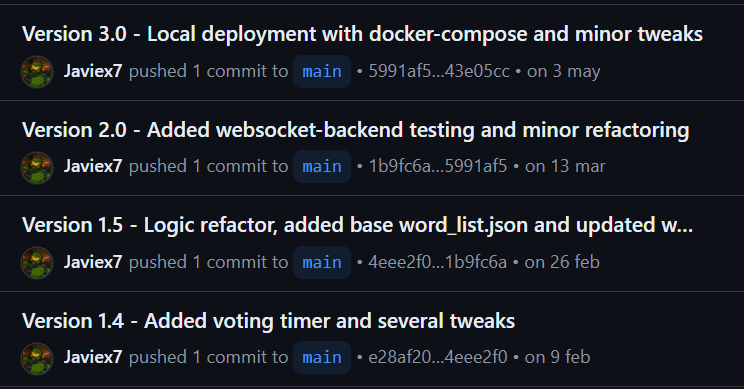
\includegraphics[width=\textwidth,clip=true]{res_commits.png}
	\caption{Aportaciones al repositorio de GitHub}
	\label{fig:res_commits}
\end{figure}

Esta metodología ha demostrado ser efectiva para este tipo de proyecto, ya que permite un avance progresivo y detallado,
evitando la acumulación de muchas tareas. Además, al planificar con visión a futuro, la aplicación ha crecido de manera sólida
y constante, sin necesidad de realizar cambios radicales.
